\chapter{MeshChat}
Meshchat is a prototype application designed to deliver messages to as many clients as possible without the need for centralized infrastructure.
The first step in the design of such an application is to design a protocol that will define how the messages will be distributed.
Once a basic idea of protocol is in place it is necessary to understand whether or not the communication primitives provided by Bluetooth on Android are suitable to implement the protocol.
The following chapter will describe the first iteration of the protocol, the test performed to verify the soundness of the basic primitives and the issues encountered while developing the tests.

\section{Primitives}
The API provided by the Android system to work with Bluetooth only allow access to the RFCOMM layer of the protocol stack.
Since RFCOMM emulates a serial connection it does not support sending a packet to more than one device at a time.
In order to simulate a multicast transmission the application must send messages to each of its peers individually.

An application can also discover nearby devices by requesting an inquiry scan.
The inquiry scan is a very intensive operation that consumes a lot of battery power and degrades the transmission performance of the Bluetooth radio.
Because of the drawbacks it is always best to perform short inquiry scans separated by a few minutes of pause.

\section{Performance testing}
To investigate whether or not the primitives provided were suitable for the task we implemented 3 synthetic benchmarks designed to closely match real world scenarios.

\subsection{Devices}
Different devices were employed for testing. Table \ref{table:devices-used} provides a correspondence between names used in the graphs and the mark and model of the devices 
used.

\begin{table}[h]
\centering
\caption{Devices used for performance testing}
\label{table:devices-used}
\begin{tabular}{lllll}
\hline
Name          & Manufacturer      & Model name    \\ \hline
Nexus 5       & Google            & Nexus 5       \\
Nexus 7       & Google            & Nexus 7       \\
OnePlus One 1 & OnePlus           & One           \\
OnePlus One 2 & OnePlus           & One           \\
Redmi         & Xiaomi            & Redmi 2       \\ 
\hline
\end{tabular}
\end{table}

\subsection{Throughput}
This benchmark was designed to test the transmission performance of Bluetooth in the context of a long lasting connection to a single other device such as the exchange of a picture or video.
Transmission performance is defined in terms of bytes transferred per second.

A single run of the test involved two devices: a server which sent packets of a predefined size and a client which received the packets and computed the time necessary to receive them.
The test was then run between each pair of devices and the results are shown in Figure \ref{figure:throughput}.

\begin{figure}[ht!]
  \centering
  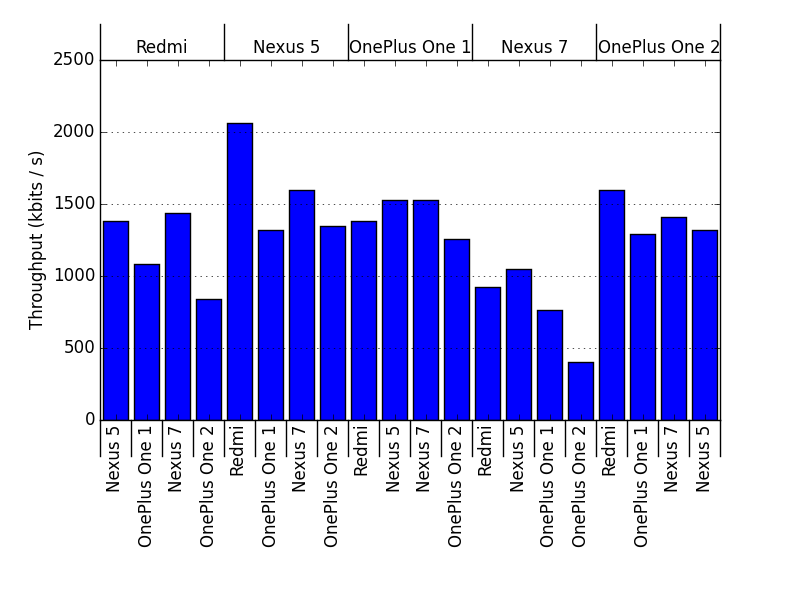
\includegraphics[width=1.0\textwidth]{img/throughput.png} 
  \caption{KBytes received per second. Devices on the top are servers while devices on the bottom are clients.}
  \label{figure:throughput}
\end{figure}

\subsection{Round trip time}
In an application designed to allow people to communicate, the time a message takes to be delivered is an important parameter.
In order to 


\begin{figure}[ht!]
  \centering
  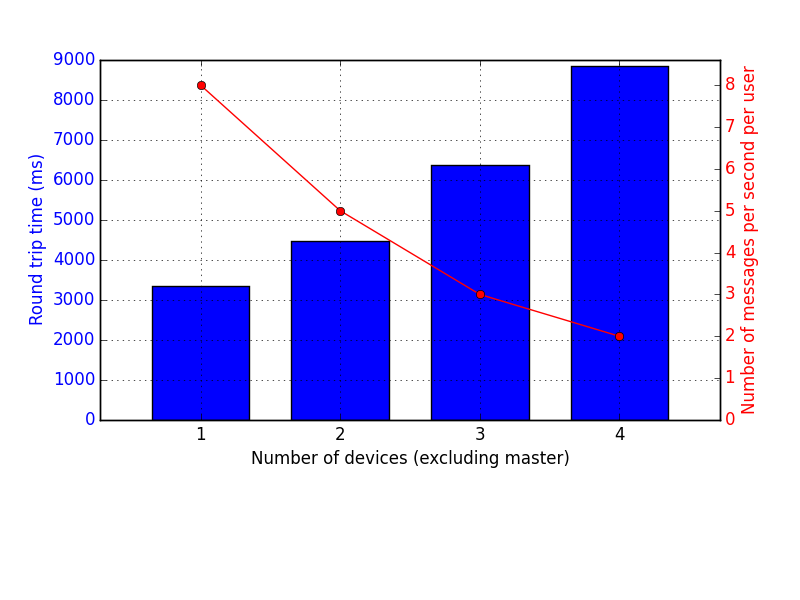
\includegraphics[width=1.0\textwidth]{img/messages_per_second.png} 
  \caption{Estimate of Round Trip Time and Messages per second rate}
  \label{figure:messages-per-second}
\end{figure}
